%%%%%%%%%%%%%% 04/03/2020 %%%%%%%%%%%%%%%% 
\subsection*{04/03/2020}

\subsubsection{Days Aim}
\begin{itemize}
    \item Finish Z 
    \item Finish Higgs
\end{itemize}

\subsubsection{Days Summary}
\begin{itemize}
    \item Made cuts on Higgs invariant mass to ensure pairs were matched
    \item Reduced higgs background
    \item Plotted cross section against changing inv mass cut to estimate systematic uncertainty 
\end{itemize}


\subsubsection*{09:00 - Morning planning call}
\subsubsection*{09:30 - Lead BG - Plot Higgs invariant mass with $100 GeV < m_{llll < 150 GeV}$}
Plot Higgs invariant mass with $100 GeV < m_{llll < 150 GeV}$.
\\
Cuts used in Fig.\ref{}
\begin{lstlisting}
    lepCut ="(" + "lep_n==4" + "&&" + t_c_cut + "&&" + lep_pair_inv_mass_cut + ")"
    
    t.Draw("inv_mass_4 >> h_inv_mass_4(50,100e3,150e3)", weighting + "*" + lepCut)
\end{lstlisting}
\begin{figure}[h!]
    \centering
	\includegraphics[width=0.85\linewidth]{04-03-2021/}
    \caption{}
    \label{}
\end{figure}

% Attempt to estimate the systematic uncertainty on $\sigma (Z \rightarrow ee)$
%%%  $\sigma (Z \rightarrow ee)$ varying invariant mass lower bound
%%%%%%%%%%%%% 10:00 %%%%%%%%%%%%% -  $\sigma (Z \rightarrow ee)$ varying invariant mass lower bound
\subsubsection*{10:00 - $\sigma (Z \rightarrow ee)$ }
Increase the upper bound on invaraint mass to $m_{ee} > 80 GeV$.
\\
Cuts used:
\begin{lstlisting}
    (invar-mass > 80 GeV) && (invar-mass < 150 GeV) && (pt > 35 GeV) && (ptcone < 5.8 GeV) && (etcone < 6 GeV) && (etcone > -2 GeV)
\end{lstlisting}



%%%%%%%%%%%%% 10:20 %%%%%%%%%%%%% -  $\sigma (Z \rightarrow ee)$ varying invariant mass lower bound
\subsubsection*{10:20 - $\sigma (Z \rightarrow ee)$ }
Increase the upper bound on invaraint mass to $m_{ee} > 90 GeV$.
\\
Cuts used:
\begin{lstlisting}
(invar-mass > 90 GeV) && (invar-mass < 150 GeV) && (pt > 35 GeV) && (ptcone < 5.8 GeV) && (etcone < 6 GeV) && (etcone > -2 GeV)
\end{lstlisting}

%%%%%%%%%%%%% 10:37 %%%%%%%%%%%%% -  $\sigma (Z \rightarrow ee)$ varying invariant mass lower bound
\subsubsection*{10:37 - $\sigma (Z \rightarrow ee)$ }
Increase the upper bound on invaraint mass to $m_{ee} > 100 GeV$.
\\
Cuts used:
\begin{lstlisting}
(invar-mass > 100 GeV) && (invar-mass < 150 GeV) && (pt > 35 GeV) && (ptcone < 5.8 GeV) && (etcone < 6 GeV) && (etcone > -2 GeV)
\end{lstlisting}

%%%%%%%%%%%%% 10:46 %%%%%%%%%%%%% -  $\sigma (Z \rightarrow ee)$ varying invariant mass lower bound
\subsubsection*{10:46 - $\sigma (Z \rightarrow ee)$ }
Increase the upper bound on invaraint mass to $m_{ee} > 60 GeV$.
\\
Cuts used:
\begin{lstlisting}
(invar-mass > 60 GeV) && (invar-mass < 150 GeV) && (pt > 35 GeV) && (ptcone < 5.8 GeV) && (etcone < 6 GeV) && (etcone > -2 GeV)
\end{lstlisting}

%%%%%%%%%%%%% 14:42 %%%%%%%%%%%%%
\subsubsection{14:42 - Plot Higgs invariant mass with tighter cuts in $m_{ll}$ for off shell z boson}
Decrease the upper bound on the invariant mass of the virtual Z boson to $m_{ll} < 60GeV$ whilst keeping the bound on the on shell bound to be $60GeV < m_{ll} < 150 GeV$
\\
Cuts used in Fig.\ref{fig:14:42_04-03-21}:
\begin{lstlisting}
    # Allowed processes: ee mumu, ee ee, mumu mumu
    # For an allowed process, the sum of charge * type == 0 
    t_c_b = "(lep_charge[{0}] * lep_type[{0}])"  
    t_c = ""
    
    for i in range(4):
        if i != 0:
            t_c += " + "
        t_c += t_c_b.format(i)

    t.SetAlias("t_c_sum", t_c)
    t_c_cut = "t_c_sum == 0"
    
    # Invariant mass of the two lepton pairs 
    # one pair has to be within the mass width of Z boson.
    # with another which does not (the virtual z boson)
    # Will have mulitple pair cominations so need to calculate invariant mass for all possible combinations (combinatorics)

    lep2_invar_mass_str = "sqrt(2*lep_pt[{0}]*lep_pt[{1}]*(cosh(lep_eta[{0}]-lep_eta[{1}])-cos(lep_phi[{0}]-lep_phi[{1}])))"

    t_c_pair = "(lep_charge[{0}] * lep_type[{0}]) + (lep_charge[{1}] * lep_type[{1}])"

    lep_pair_inv_mass_cut = ""

    i = 0
    for j in range(1, 4):
        for k in range(1, 3):
            for l in range(2, 4):
                if j != k and j != l and k != l and k < l:
                    print(i,j,k,l)
                    if not (j == 1 and k == 2 and l == 3):
                        lep_pair_inv_mass_cut += " || "
                    lep_pair_inv_mass_cut += lep2_invar_mass_str.format(i, j) + " > 60e3 && " + lep2_invar_mass_str.format(i, j) + " < 150e3 && " + lep2_invar_mass_str.format(k,l) + " < 60e3" + " && " + t_c_pair.format(i, j) + " == 0 && " + t_c_pair.format(k,l) + " == 0" + " || " + lep2_invar_mass_str.format(k, l) + " > 60e3 && " + lep2_invar_mass_str.format(k, l) + " < 150e3 && " + lep2_invar_mass_str.format(i,j) + " < 60e3" + " && " + t_c_pair.format(k, l) + " == 0 && " + t_c_pair.format(i, j) + " == 0"
    
    # Calulcate invariant mass of Higgs from the 4 leptons.
    x = "2 * lep_pt[{0}] * lep_pt[{1}]*(cosh(lep_eta[{0}]-lep_eta[{1}]) - cos(lep_phi[{0}]-lep_phi[{1}]))"
    s = ""

    for i in range(4):
        for j in range(i+1, 4):
            if not (i == 0 and j == 1):
                s += "+"
            s += x.format(i, j)
 
    t.SetAlias("s", s)
    t.SetAlias("inv_mass_4", "sqrt(s)")

    lepCut ="(" + "lep_n==4" + "&&" + t_c_cut + "&&" + lep_pair_inv_mass_cut + ")"
    
    t.Draw("inv_mass_4 >> h_inv_mass_4(50,100e3,140e3)", weighting + "*" + lepCut)
    
\end{lstlisting}

\begin{figure}[h!]
    \centering
	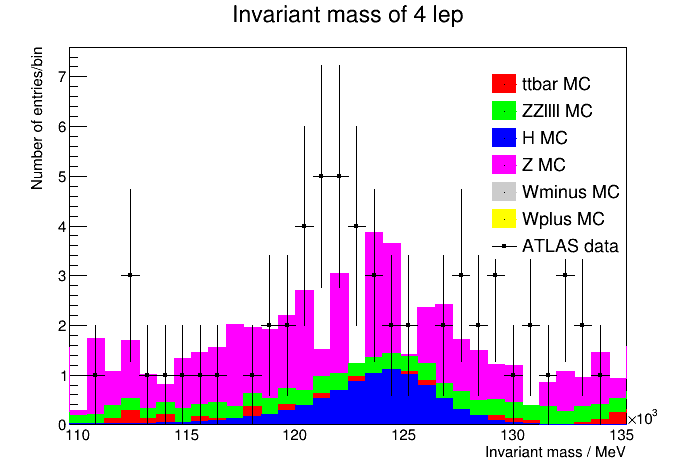
\includegraphics[width=0.85\linewidth]{plots/04-03-2021/14-42.png}
    \caption{Invariant mass plot using ATLAS and Higgs MC data.  Cuts: lep-n == 4, only allowed end products: == e+e- mu+mu-, e+e-e+e-, mu+mu- mu+mu-, with one lepton pair with invariant mass of $60 GeV < m_{ll} < 150 GeV$ and the other $m_{ll} < 60 GeV$}
    \label{fig:14:42_04-03-21}
\end{figure}



%%%%%%%%%%%%% 15:30 %%%%%%%%%%%%%
\subsubsection*{15:30 - Cross section of Z -> ee - calculating the syst. uncert}
\begin{figure}[h!]
    \centering
	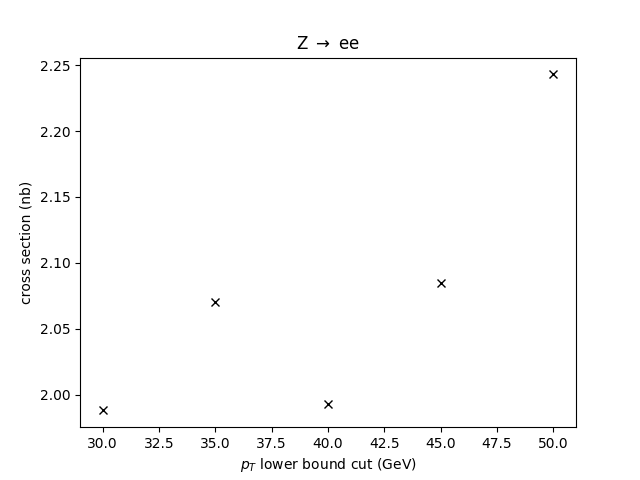
\includegraphics[width=0.85\linewidth]{plots/04-03-2021/15-45_04-03-21.png}
    \caption{The cross section of Z -> ee using final cuts but varying the lower bound on the transverse momentum between 30 GeV and 50 GeV.  (final cuts = $(invar-mass > 70 GeV) && (invar-mass < 150 GeV) && (pt > 35 GeV) && (ptcone < 5.8 GeV) && (etcone < 6 GeV) && (etcone > -2 GeV)$)}
    \label{fig:15:30_04-03-21}
\end{figure}
From Fig.\ref{fig:15:30_04-03-21} there seems to have the cross section about stable between 30 GeV and 45 GeV. 
\\
Therefore take the range of cross section to be the value at 30 GeV and at 45 GeV
\\
$2.085 - 1.988 = 0.098 (nb)$
\\
So for the systematic uncertainty for $\sigma (Z \rightarrow) ee$ using the cuts $ (invar-mass > 70 GeV) && (invar-mass < 150 GeV) && (pt > 35 GeV) && (ptcone < 5.8 GeV) && (etcone < 6 GeV) && (etcone > -2 GeV) $ is 0.049 nb


%%%%%%%%%%%%% 16:19 %%%%%%%%%%%%%
\subsubsection*{16:19 - Plot the pT of Higgs}
Plot the transverse momentum of one of the the leptons produced in the Higgs process.
\\
Cuts used in Fig.\ref{fig:16:19_04-03-21}:
\begin{lstlisting}
    # Allowed processes: ee mumu, ee ee, mumu mumu
    # For an allowed process, the sum of charge * type == 0 
    t_c_b = "(lep_charge[{0}] * lep_type[{0}])"  
    t_c = ""
    
    for i in range(4):
        if i != 0:
            t_c += " + "
        t_c += t_c_b.format(i)

    t.SetAlias("t_c_sum", t_c)
    t_c_cut = "t_c_sum == 0"
    
    
    # Generate invariant mass range cut (110 GeV < m_{llll} < 133 GeV)
    invar_mass_cut = "(inv_mass_4 > 110e3 && inv_mass_4 < 133e3)"
    
    # Invariant mass of the two lepton pairs 
    # one pair has to be within the mass width of Z boson.
    # with another which does not (the virtual z boson)
    # Will have mulitple pair cominations so need to calculate invariant mass for all possible combinations (combinatorics)

    lep2_invar_mass_str = "sqrt(2*lep_pt[{0}]*lep_pt[{1}]*(cosh(lep_eta[{0}]-lep_eta[{1}])-cos(lep_phi[{0}]-lep_phi[{1}])))"

    t_c_pair = "(lep_charge[{0}] * lep_type[{0}]) + (lep_charge[{1}] * lep_type[{1}])"

    lep_pair_inv_mass_cut = ""

    i = 0
    for j in range(1, 4):
        for k in range(1, 3):
            for l in range(2, 4):
                if j != k and j != l and k != l and k < l:
                    print(i,j,k,l)
                    if not (j == 1 and k == 2 and l == 3):
                        lep_pair_inv_mass_cut += " || "
                    lep_pair_inv_mass_cut += lep2_invar_mass_str.format(i, j) + " > 60e3 && " + lep2_invar_mass_str.format(i, j) + " < 150e3 && " + lep2_invar_mass_str.format(k,l) + " < 60e3" + " && " + t_c_pair.format(i, j) + " == 0 && " + t_c_pair.format(k,l) + " == 0" + " || " + lep2_invar_mass_str.format(k, l) + " > 60e3 && " + lep2_invar_mass_str.format(k, l) + " < 150e3 && " + lep2_invar_mass_str.format(i,j) + " < 60e3" + " && " + t_c_pair.format(k, l) + " == 0 && " + t_c_pair.format(i, j) + " == 0"
    
    # Calulcate invariant mass of Higgs from the 4 leptons.
    x = "2 * lep_pt[{0}] * lep_pt[{1}]*(cosh(lep_eta[{0}]-lep_eta[{1}]) - cos(lep_phi[{0}]-lep_phi[{1}]))"
    s = ""

    for i in range(4):
        for j in range(i+1, 4):
            if not (i == 0 and j == 1):
                s += "+"
            s += x.format(i, j)
 
    t.SetAlias("s", s)
    t.SetAlias("inv_mass_4", "sqrt(s)")

    lepCut ="(" + "lep_n==4" + "&&" + t_c_cut + "&&" + lep_pair_inv_mass_cut + "&&" + invar_mass_cut + ")"
    
    t.Draw("lep_pt[0] >> h_lep_pt_4(80,0e3,200e3)", weighting + "*" + lepCut)
\end{lstlisting}


\begin{figure}[h!]
    \centering
	\includegraphics[width=0.85\linewidth]{04-03-2021/}
    \caption{Transverse momentum of one of the leptons produced by an event with 4 leptons produced (possible Higgs candidate).} 
    \label{fig:16:19_04-03-21}
\end{figure}


%%%%%%%%%%%%%%%%%%%%%%%%%%%%%%%%%%%%%%%%%%%%%%%%%%%%%%%%%%%%%%%%%%%%%%%%%%%%%%%%%%%%%%%%%%%%%%%%%%%%%%%%%%%%%%%%%%%%%%%%%%%%%%%%%%%%%%%%%%%%%%%%%%%%%%%%%%%%%%%%%%%%%%%%%%%%%%%%%%%%%%%%%%%%%%%%%%%%%%%%%%%%%%%%%%%%%%%%%%%%%%%%%%%%%%%%%%%%%%%%%%%%%%%%%%%%%%%%%%%%%%%%%%%%%%%%%%%%%%%%%%%%%%%%%%%%%%%%%%%%%%%%%%%%%%%%%%%%%%%%%%%%%%%%%%%%%%%%%%%%%%%%%%%%%%%%%%%%%%%%%%%%%%%%%%%%%%%%%%%%%%%%%%%%%%%%%%%%%%%%%%%%%%%%%%%%%%%%%%%%%%%%%%%%%%%%%%%%%%%%%%%%%%%%%%%%%%%%%%%%%%%%%%%%%%%%%%%%%%%%
\begin{figure}[h!]
    \centering
    \begin{minipage}{0.5\textwidth}
        \centering
        \includegraphics[width=\linewidth]{plots/02-03-2021/}
        (A)
    \end{minipage}\hfill
    \begin{minipage}{0.5\textwidth}
        \centering
        \includegraphics[width=\linewidth]{plots/02-03-2021/}
        (B)
    \end{minipage}
    \caption{(A)  (B)}
    \label{}
\end{figure}